\documentclass[hyperref={pdfpagelabels=false}]{beamer}
\graphicspath{{assets/}}
\usepackage{lmodern}
\usetheme{CambridgeUS}
\beamertemplatenavigationsymbolsempty


\renewcommand*{\bibfont}{\tiny}
 
\usepackage{media9}
\usepackage{booktabs}
\usepackage{graphics}

%% \usepackage{appendixnumberbeamer}
%% \expandafter\def\expandafter\insertshorttitle\expandafter{%
%%   \insertshorttitle\hfill\insertframenumber\,/\,\inserttotalframenumber}

\usepackage[backend=biber]{biblatex}
\addbibresource{assets/references.bib}

% Custom colors
% \usepackage{xcolor}
% http://www.computerhope.com/htmcolor.htm
% \definecolor{light blue}{HTML}{AAAAFF}
% \definecolor{light green}{HTML}{AAAAFF}

\makeatletter
\definecolor{mybackground}{HTML}{82CAFA}
\definecolor{myforeground}{HTML}{0000A0}

\setbeamercolor{normal text}{fg=black,bg=gray!10!white}
\setbeamercolor{alerted text}{fg=red}
\setbeamercolor{example text}{fg=black}

\setbeamercolor{background canvas}{fg=mybackground, bg=white}
\setbeamercolor{background}{fg=myforeground, bg=mybackground}

\setbeamercolor{palette primary}{fg=black, bg=blue!20!white}
\setbeamercolor{palette secondary}{fg=black, bg=blue!40!white}
\setbeamercolor{palette tertiary}{fg=black, bg=blue!60
  !white}
\setbeamercolor{frametitle}{fg=black, bg=gray!20!white}
\setbeamercolor{title}{fg=black, bg=gray!20!white}

\setbeamercolor{part title}{fg=black, bg=blue!60!white}
\makeatother




\title[R\=aga Classification]{Carnatic R\=aga Classification Using\\Convolutional Neural Networks}  
\author[Andr\'es Fern\'andez Rodr\'iguez]{Andr\'es Fern\'andez Rodr\'iguez}
\institute[]{Goethe Universit\"at Frankfurt am Main}
\date{October 13, 2017} 
\begin{document}
\titlegraphic{
\includegraphics[scale=0.15]{goethe-logo.png}}
     {\frame \titlepage}



     \begin{frame}
       \frametitle{Table of contents}
       \tableofcontents
     \end{frame}



     %%%%%%%%%%%%%%%%%%%%%%%%%%%%%%%%%%%%%%%%%%%%%%%%%%%%%%%%%%%%%%%%%%%%%%%%%%%%%%%%%%%%%%%%
     \section{About Carnatic Music}
     \frame{\sectionpage}
     %%%%%%%%%%%%%%%%%%%%%%%%%%%%%%%%%%%%%%%%%%%%%%%%%%%%%%%%%%%%%%%%%%%%%%%%%%%%%%%%%%%%%%%%

     % \subsection{Context}
     %%%%%%%%%%%%%%%%%%%%%%%%%%%%%%%%%%%%%%%%%%%%%%%%%%%%%
     \begin{frame}
       \frametitle{General Aspects of Carnatic Music}
       \begin{itemize}[<.->]
       \item Oral tradition from South India (organized in schools called ghar\=an\=a)
       \item Specialized ensemble of few soloists with predominance of melody
       \item Four relevant elements: r\=aga, t\=ala, composition and improvisation
         \begin{itemize}[<.->]
         \item \textbf{R\=aga} is the melodic framework
         \item T\=ala is the rhythmic framework
         \item Compositions and improvisation techniques depend on school/person
         \end{itemize}
       \item Delivered in a concert (1-2 hours), playing several pieces (20-30 min)
       \end{itemize}

       \begin{center}
         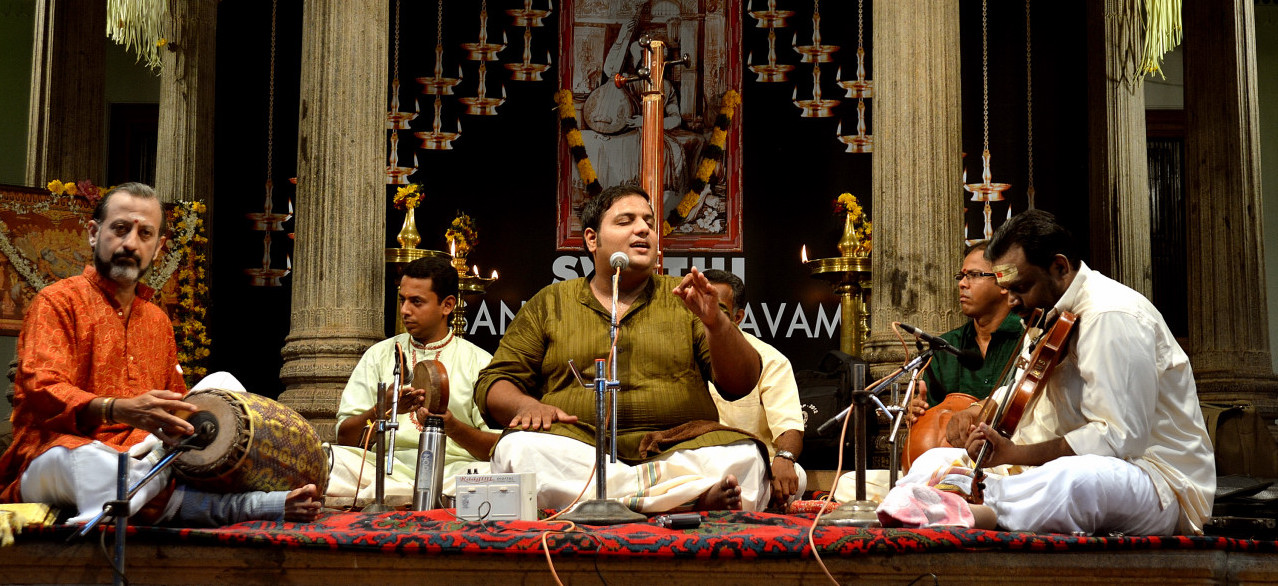
\includegraphics[scale=0.15]{carnatic_ensemble.png}
                         {\scriptsize \\A traditional carnatic ensemble (from \cite[p.17]{gulati})}
       \end{center}
     \end{frame}

     % \subsection{The Melodic Framework}
     %%%%%%%%%%%%%%%%%%%%%%%%%%%%%%%%%%%%%%%%%%%%%%%%%%%%%
     \begin{frame}
       \frametitle{R\=aga Building Blocks}
       Each r\=aga has a specific set of the following melodic elements:
       \vspace{2mm}
       \begin{itemize}
       \item \textbf{Svaras}: The basic pitches, defined with respect to the fundamental
       \item \textbf{Gamakas}: Ornaments applied to the svaras
       \item \textbf{Ny\=as svaras} The pitches that can be held longer
       \item \textbf{\=Ar\=ohana and Avr\=ohana}: ascending and descending melodic patterns, respectively
       \item \textbf{Phrases and Chalans}: Phrases are traditional {\it licks}, chalans are their underlying structure (a phrase without the gamakas)
       \end{itemize}

       \begin{alertblock}{Implicit features}
         Due to improvisatoric+oral nature of the repertoire, this building blocks present a high variance: \textbf{the svaras and chalans are conceptual and never appear without Gamakas}
       \end{alertblock}
     \end{frame}

     %%%%%%%%%%%%%%%%%%%%%%%%%%%%%%%%%%%%%%%%%%%%%%%%%%%%%
     \begin{frame}
       \frametitle{R\=aga Recognition Example}
       Example of the svara set identification for three different r\=agas:
       \begin{center}
         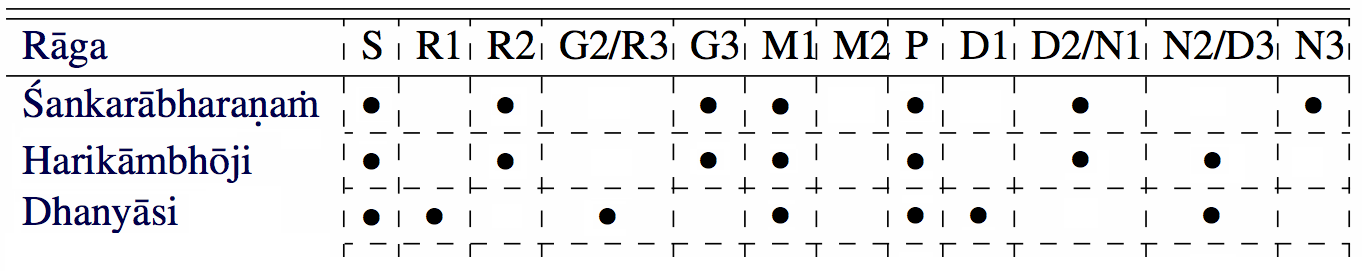
\includegraphics[scale=0.25]{svaras_example.png}
         \\{\scriptsize The svara set of three diferent r\=agas (from \cite[p.244]{gulati})}
       \end{center}

       \begin{itemize}
       \item Audio 1 is a clear example of the first r\=aga
         
       \item Audio 2 is a clear example of the last r\=aga, contrasting with A1
       \item Audio 3 is a clear example of the middle r\=aga, note similarity with A1
       \item Audio 4 is an ambiguous example, since the {\it Ni} svara never appears in the first minute
       \end{itemize}
     \end{frame}



     %%%%%%%%%%%%%%%%%%%%%%%%%%%%%%%%%%%%%%%%%%%%%%%%%%%%%%%%%%%%%%%%%%%%%%%%%%%%%%%%%%%%%%%%
     \section{Related Work on R\=aga Classification}
     \frame{\sectionpage}
     %%%%%%%%%%%%%%%%%%%%%%%%%%%%%%%%%%%%%%%%%%%%%%%%%%%%%%%%%%%%%%%%%%%%%%%%%%%%%%%%%%%%%%%%



     %%%%%%%%%%%%%%%%%%%%%%%%%%%%%%%%%%%%%%%%%%%%%%%%%%%%%
     \begin{frame}
       \frametitle{The CompMusic Project}
       \begin{itemize}
       \item Multi-team project hosted at the UPF Barcelona (\cite{serra-comp11}, \cite{serra-comp14})
       \item Effort towards data-driven and culture-aware approaches in the Music Information Retrieval field
       \item Compilated and curated an open \textbf{carnatic corpus} with around 2500 recordings, labeled with r\=aga, form, artists and t\=ala among others\cite{indian-corpora}
       \item On the r\=aga domain: at the moment of downloading, 2050 recordings (over 425 hours) distributed over 220 r\=agas, the most represented one having over 60 recordings and 30 hours
       \item     The R\=aga Recognition Dataset (\boldmath{$RRD_{CMD}$}) is a test subset of the carnatic corpus covering 40 r\=agas, with 12 recordings each, and around 124 hours of total duration\cite[p.84]{gulati}. ``{\it The largest and most comprehensive ever for this task}''\cite[p.183]{gulati}
       \end{itemize}


     \end{frame}


     %%%%%%%%%%%%%%%%%%%%%%%%%%%%%%%%%%%%%%%%%%%%%%%%%%%%%
     \begin{frame}
       \frametitle{Relevant Approaches}
       In his 2016 dissertation, Sankalp Gulati develops two model and tests them on the $RRD_{CMD}$ subset. After extracting the melody line:
       \vspace{3mm}
       \begin{itemize}[<.->]
       \item Vector Space Modelling (VSM)\cite[p.179]{gulati}, inspired in text processing: phrases$\leftrightarrow$words, r\=agas$\leftrightarrow$topics, recordings$\leftrightarrow$documents
         \begin{enumerate}[<.->]
         \item clustering the phrases into a dictionary of building blocks\cite[p.204]{gulati}
         \item considering the recording a text-like vector of such blocks
         \item applying a classifier on top (semi-supervised)
         \item Accuracy below SoTA (67.3\%). Sensitive to allied r\=agas
         \end{enumerate}
         \vspace{3mm}
       \item Time-Delayed Melody Surface (TDMS)\cite[p.192]{gulati}
         \begin{enumerate}[<.->]
         \item normalize around tonic and wrap around octaves to get $\eta$ distinct frequency bins
         \item scroll the normalized melody with two points of a short, fixed delay between them and add their pitch relations to an $\eta\times\eta$ histogram
         \item post-process and apply a classifier on top (semi-supervised)
         \item Accuracy well above SoTA (86.7\%)
         \end{enumerate}
       \end{itemize}
     \end{frame}


     \begin{frame}
       \frametitle{Characteristics of TDMS Representation}
       \textbf{Compact, fast to compute, continuous, meaningful, performative.}
       \vspace{4mm}
       \begin{columns}
         \column{0.5\linewidth}
         \centering
          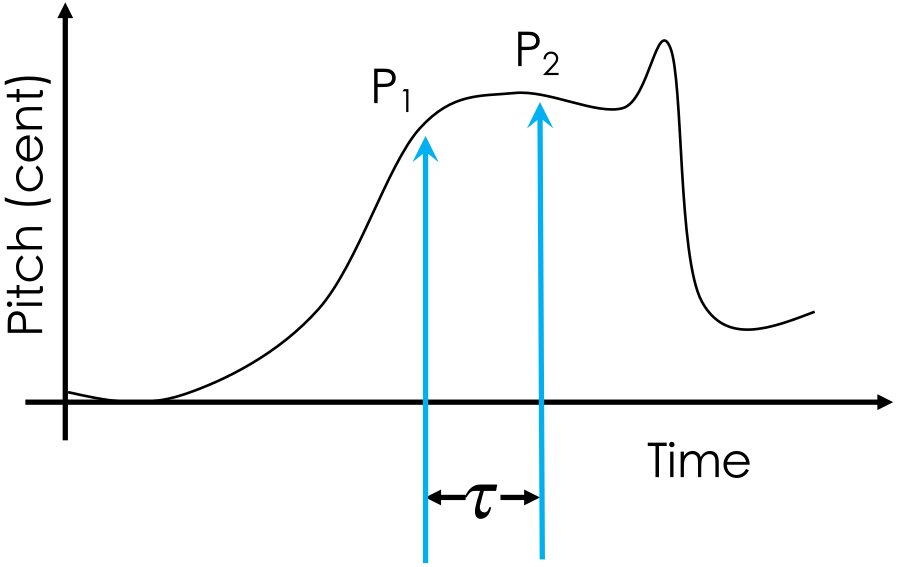
\includegraphics[scale=0.2]{tdms_line.png}
         \\\scriptsize{The melodic contour of a piece is scrolled with a fixed, small delay $\tau$ and the $(P_1, P_2)$ relations added to the TDMS (from \cite[p.163]{gulati-slides})}
         \column{0.5\linewidth}
         \centering
          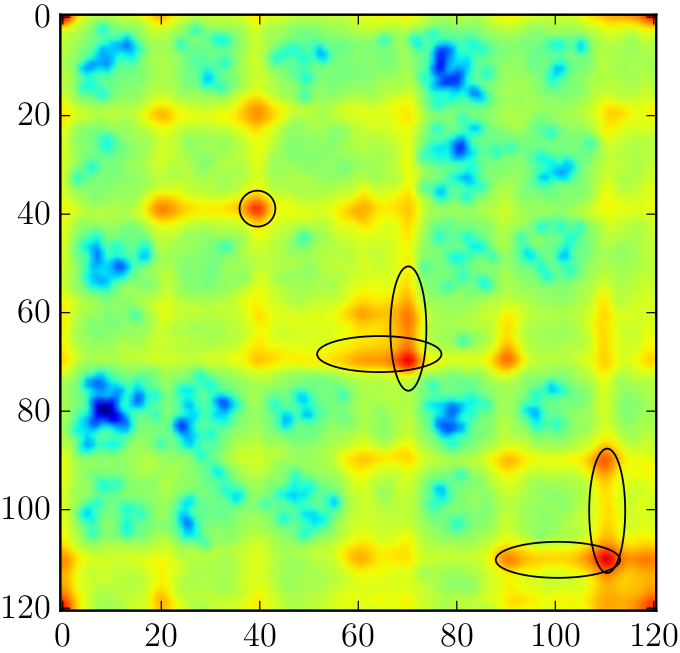
\includegraphics[scale=0.2]{tdms.png}
         \\\scriptsize{A TDMS of a a music piece in r\=aga Yaman, with the octave divided in 120 bins. The frequent ny\=as and gamakas can be intuitively seen (from \cite[p.170]{gulati-slides})}
       \end{columns}
     \end{frame}




     %%%%%%%%%%%%%%%%%%%%%%%%%%%%%%%%%%%%%%%%%%%%%%%%%%%%%%%%%%%%%%%%%%%%%%%%%%%%%%%%%%%%%%%%
     \section{Approach and Task Definition}
     \frame{\sectionpage}
     %%%%%%%%%%%%%%%%%%%%%%%%%%%%%%%%%%%%%%%%%%%%%%%%%%%%%%%%%%%%%%%%%%%%%%%%%%%%%%%%%%%%%%%%


     %%%%%%%%%%%%%%%%%%%%%%%%%%%%%%%%%%%%%%%%%%%%%%%%%%%%%
     \begin{frame}
       \frametitle{Approach and Problem Definition}
       The improvement in performance by the TDMS model is given under the following conditions:
       \begin{itemize}
       \item Most of the carnatic corpus' data remains unused
       \item Semi-supervised methods were applied to fully labeled data
       \item Melody extraction supposes a very drastic compression of the data
       \item The time-frequency relations of the melody contour are enough to capture the r\=agas' features
       \end{itemize}
       \vspace{5mm}
       This, added to \textbf{my assumptions} that \textbf{the corpus is sizable}\cite[p.iii]{andres-bachelor}, and that the \textbf{arguably related field of Music Genre Recognition}\cite[p.17]{andres-bachelor} (MGR) presents a lot of successful, recent research applying supervised end-to-end methods, made interesting and feasible the following
       \begin{block}{Task:}
         Perform carnatic r\=aga classification using supervised, end-to-end convolutional neural networks (CNNs) from the MGR field's SoTA.
       \end{block}
     \end{frame}



     %%%%%%%%%%%%%%%%%%%%%%%%%%%%%%%%%%%%%%%%%%%%%%%%%%%%%%%%%%%%%%%%%%%%%%%%%%%%%%%%%%%%%%%%
     \section{Related Work on End-to-end Music Classification}
     \frame{\sectionpage}
     %%%%%%%%%%%%%%%%%%%%%%%%%%%%%%%%%%%%%%%%%%%%%%%%%%%%%%%%%%%%%%%%%%%%%%%%%%%%%%%%%%%%%%%%


     %%%%%%%%%%%%%%%%%%%%%%%%%%%%%%%%%%%%%%%%%%%%%%%%%%%%%
     \begin{frame}
       \frametitle{The MGR Field}
       MGR is also a part of the MIR field. Main considerations\cite[p.17]{andres-bachelor}:
       \begin{itemize}
       \item A straightforward top-bottom definition of genre is also impossible. Many features apart from time and frequency (timbre, lyrics...)
       \item Also lack of unified\&global criteria and data. Most of the research is western-based, around labeled song-sets like the Million Song Dataset (MSD)
       \item Apart from waveforms, popular representations are STFT and MFCC (so-called time/frequency representations, because they capture the sound intensity through time for specific frequency bands)
       \end{itemize}
       \centering
          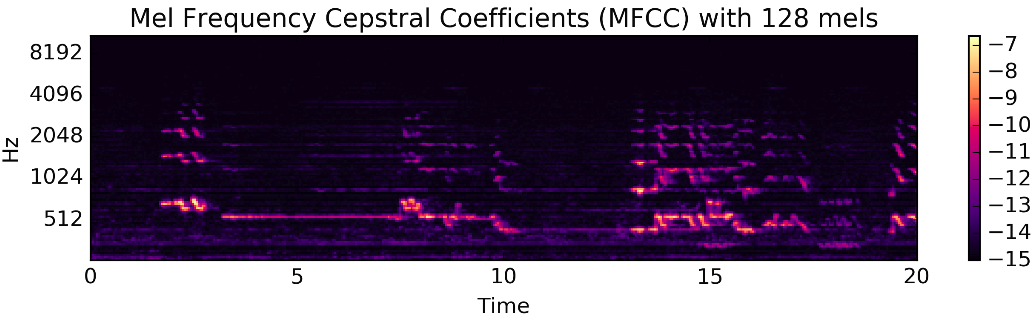
\includegraphics[scale=0.26]{flute_melgram.png}
         \\\scriptsize{the beginning of a piece in Kaly\=a\d{n}i r\=aga: {\it Sikkil Sisters -- Nijadasa Varada} (audio 5)}
     \end{frame}

     %%%%%%%%%%%%%%%%%%%%%%%%%%%%%%%%%%%%%%%%%%%%%%%%%%%%%
     \begin{frame}
       \frametitle{Recent MGR Approaches}
       Notable work has been developed in \cite{choi-fcn}, \cite{choi-crnn}, \cite{choi-robustness}, \cite{choi-explaining} and \cite{convtransfer}:
       \begin{itemize}
       \item MSD (training: 201,680 --  validation: 12,605 -- test: 25,940 songs)
       \item Multi-tagging on top-50 tags including genres (rock, pop, funk) and moods (sad, happy, chill)
       \item FCN4 Achieved 0.894 AUC-ROC on the test subset
       \end{itemize}
          \centering
          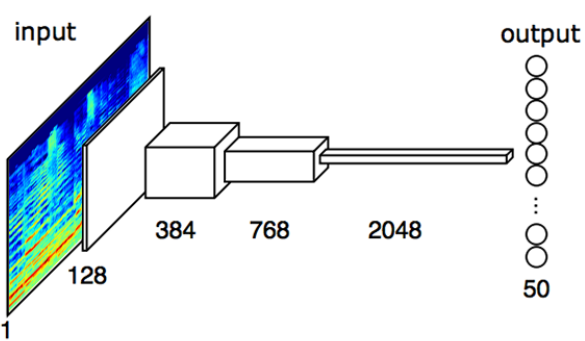
\includegraphics[scale=0.3]{fullyconv.png}
         \\\scriptsize{One of the fully-convolutional neural architectures (FCN4) proposed in \cite{choi-fcn}. The numbers indicate the number of feature maps (i.e. channels)}
     \end{frame}

     %%%%%%%%%%%%%%%%%%%%%%%%%%%%%%%%%%%%%%%%%%%%%%%%%%%%%
     \begin{frame}[allowframebreaks]
       \frametitle{Supervised Learning with NNs -- Highlights}
       \begin{itemize}
       \item Neural networks are models that alternate linear with non-linear transformations  to provide the so-called \textbf{hypothesis} $h_\theta(x)$, based on some set of \textbf{parameters} $\theta$. CNNs are NNs that have at least one convolution
       \item For a labeled \textbf{sample} $(x_i, y_i)$, given a \textbf{cost function} $J(h(x_i), y_i)$ between its \textbf{label} and the corresponding hypothesis, it is possible to measure the error of the network. The \textbf{learning} process consists in alter the parameters to minimize this error
       \item $J$ is usually non-convex, so it is optimized using the \textbf{gradient descent} algorithm: $\theta^{(t+1)} := \theta^{(t)} - \alpha \frac{\partial}{\partial \theta} J(X, Y)$, that follows the derivative of $J$ downwards proportionally to $\alpha$, the \textbf{learning rate}
       \item Once the network memorizes the training data, stops learning from it. This lack of generalization ability is known as \textbf{overfitting}, and the measures to prevent it as \texbf{regularization}. Two important regularization techniques are \textbf{weight decay} and \textbf{dropout}
       \item The size of $X, Y$ (\textbf{batch size}) is also a regularization factor. The parameters that aren't trained by the network are called \textbf{hyperparameters}, and are usually optimized by splitting the non-training data into \textbf{test} and \textbf{validation}, and doing a \textbf{grid search}
       \item CNNs usually alternate convolution with \textbf{pooling}. This combo helps to capture local features. Usually this is done several times, increasing the number of filters and decreasing their size (\textbf{repr. learning})
       \item CNNs are based on the idea of \textbf{parameter sharing}, which allow deeper architectures that perform empirically better\cite[p.202]{goodfellow}
       \end{itemize}
     \end{frame}



     %%%%%%%%%%%%%%%%%%%%%%%%%%%%%%%%%%%%%%%%%%%%%%%%%%%%%%%%%%%%%%%%%%%%%%%%%%%%%%%%%%%%%%%%
     \section{Experiments and Results}
     \frame{\sectionpage}
     %%%%%%%%%%%%%%%%%%%%%%%%%%%%%%%%%%%%%%%%%%%%%%%%%%%%%%%%%%%%%%%%%%%%%%%%%%%%%%%%%%%%%%%%

     \begin{frame}
       \frametitle{Guidelines and Implementation}
       Choosing a convolutional architecture seemed feasible to me because of the following reasons:
       \begin{itemize}
       \item CNNs should be able to ignore the background drone and percussion, as they are independent from the labeled r\=aga, and filter out the melodic contour in a way similar to the input of the VSM and TDMS algorithms
       \item Being able to detect shapes on a time/frequency representation of a melodic contour is equivalent to being sensitive to its time/frequency changes
       \item CNNs are locally limited, but Locality is explicitly recognized as an advantage in the TDMS model
       \end{itemize}
       The code was implemented on TensorFlow. A first test setup training the CNN suggested in \cite{tf-cnn} on the MNIST classification problem achieved a 98\% accuracy in less than 2 training epochs (100,000 training samples).
     \end{frame}

     \begin{frame} % commit 699a805bac7d6be2650c21c886ac52b92a220e12
       \frametitle{Rock vs. Merengue}
       After the success with the {\it vanilla} MNIST setup, I tried with some data of my own, selecting 20 songs representative of each style (audios 6 and 7), achieving a performance consistently above 90\% after two epochs. This could be due to the great timbrical differences.
       \begin{columns}
         \column{0.45\linewidth}
         \begin{table}
           \centering
           \resizebox{120}{!}{%
       \begin{tabular}{*2l}\toprule
         \bfseries Layer  & \bfseries Shape\\
         \midrule
         Input &          512\times86\times1\\
         \midrule
         Conv512x5x1x4 &    1\times82\times4\\
         Conv1x10x4x6 &         1\times73\times6\\
         Conv1x15x6x8 &        1\times59\times8\\
         Conv1x28x8x12 &        1\times40\times12\\\midrule
         FullyHidden &   40\cdot12\times 24\\
         Logits &        24 \times 2\\\midrule
       \end{tabular}}
       \\{\scriptsize The best-performing architecture among the tested ones. It has a ReLU after each convolution}
       \end{table}

         \column{0.55\linewidth}
         \centering
         \begin{tabular}{|c|c|}
         \hline
         \textbf{Hyperparameter} & \textbf{Value}\\
         \hline
         Chunk size & 1 sec \\
         \hline
         Batch size & 20 \\
         \hline
         Learning rate (SGD) & $10^{-4}$ \\
         \hline
         Weight decay rate & $0.2$ \\
         \hline
         Dropout  & none \\
         \hline
       \end{tabular}
         \\{\scriptsize The corresponding hyperparametrization}
       \end{columns}
     \end{frame}
     

\begin{frame}
  \frametitle{Augmented Carnatic Corpus -- Approach}
  After those two toy-setups, I switched to the whole corpus:
  \begin{itemize}
  \item \scriptsize To enforce intra- and inter-class balance, I applied data augmentation to the 40 classes present in the $RRD_{CMD}$ dataset by time-stretching by $unif \sim [0.7, 1.3]$
  \item \scriptsize I trained on the STFT expecting the network to adapt the exponential frequency scale to its needs, as in \cite{wavspaper}
  \end{itemize}
\vspace{-3mm}
  \begin{columns}
         \column{0.5\linewidth}
         \begin{table}
           \centering
           \resizebox{120}{!}{%
             \begin{tabular}{*2l}\toprule
               \bfseries Layer  & \bfseries Shape\\\midrule
               Input &          257\times625\times1\\\midrule
               Conv3x3x1x128 &    255\times623\times128\\%\Midrule
               MaxPool2x3    &    127\times207\times128\\\midrule
               Conv3x3x128x384 &  125\times205\times384\\%\Midrule
               MaxPool4x5 &       31\times41\times384\\\midrule
               Conv3x3x384x768 &  29\times39\times768\\%\Midrule
               MaxPool5x6 &       7\times6\times768\\\midrule
               Conv3x3x768x2048 & 3\times4\times2048\\%\Midrule
               MaxPool6x4 &       1\times1\times2048\\\midrule
               Logits(Conv1x1x40) & 1\times1\times40\\\midrule
           \end{tabular}}
         \end{table}

         \column{0.5\linewidth}
         \begin{table}
           \centering
           \resizebox{100}{!}{%
             \begin{tabular}{*2l}\toprule
               \bfseries Layer  & \bfseries Shape\\\midrule
               Input &          257\times625\times1\\\midrule
               Conv3x3x1x128 &    255\times623\times128\\%\Midrule
               MaxPool2x3    &    127\times207\times128\\\midrule
               Conv3x3x128x256 &  125\times205\times256\\%\Midrule
               MaxPool3x3 &       41\times68\times256\\\midrule
               Conv3x3x384x512 &  39\times66\times512\\%\Midrule
               MaxPool3x4 &       13\times16\times512\\\midrule
               Conv3x3x768x1024 & 11\times14\times1024\\%\Midrule
               MaxPool3x4 &       4\times3\times1024\\\midrule
               Conv3x2x768x2048 & 2\times2\times2048\\%\Midrule
               MaxPool2x2 &       1\times1\times2048\\\midrule
               Logits(Conv1x1x40) & 1\times1\times40\\\midrule
           \end{tabular}}
         \end{table}
  \end{columns}
  \vspace{-2mm}
  \\{\tiny Adaption of the \textbf{FCN4} and \textbf{FCN5} architectures\cite{choi-fcn}, respectively. There are ReLU layers between convolution and pooling. There is a ReLU and a dropout layer before the logits, in that order.}
\end{frame}


\begin{frame}
  \frametitle{Augmented Carnatic Corpus -- Some Hyperpars.\& Results}
  \begin{itemize}
  \item With Adam optimizer and initial learning rate = $10^{-4}$, batch size = 10 and chunk size = 20 seconds, grid search on $architecture\{FCN4, FCN5\} \times weightdecay\{10^{-9}, 3\cdot 10^{-9}, 10^{-8}, 3\cdot 10^{-8}, 10^{-7}, 3\cdot 10^{-7}, 10^{-6}, 3\cdot 10^{-6}, 10^{-5}, 3\cdot 10^{-4}\} \times dropout\{1, 0.95, 0.9, 0.85, 0.8, 0.75, 0.65, 0.5\}$
  \item Tested similar settings with {\it vanilla} SGD optimizer for $learningrate\{10^{-4}, 10^{-5}, ... 10^{-9}\}$
  \item Same with momentum optimizer for $momentum\{0.1, 0.2, 0.5, 0.8, 0.9\}$
    \item Modified the FCN architectures to allow different convolution depths and tested with $basedepth\{8, 16, 35, 50, 60, 80\}$
  \end{itemize}

  \begin{block}{Results}
    \scriptsize The general observed behaviour was that all the different variants overfitted with no regularization at all, but seemed unable to learn even the training data when the least amount of regularization of any kind was introduced. In any of the cases, the overall accuracy of the validation results wasn't better than random guessing.
    \end{block}
\end{frame}

\begin{frame}
  \frametitle{R\=aga Recognition Dataset -- Approach}
  \begin{itemize}
  \item Switched to the smaller MFCC representation to allow bigger batches, and also to the CQT to incorporate the logarithmic scalation of the frequency axis to the preprocessing. Also did some final tests on the plain wav files
  \item Reduced the problem space to the $RRD_{CMD}$ (hoping for denser data), first with 5 arbitrary r\=agas and then with 2 contrasting ones.
  \item Due to the observed contrast between the overfitting with no regularization and the rapid gaining of bias, I oriented my grid search to find a ``sweet spot'' between them.
  \end{itemize}
  For an example of the grid search performed, together with the thought lines behind them, see the next slide, extracted from the repository's {\it 3\_main\_pipeline.py} file.
\end{frame}

\begin{frame}
    \frametitle{$RRD_{CMD}$ -- Finetuning Example}
    \centering
    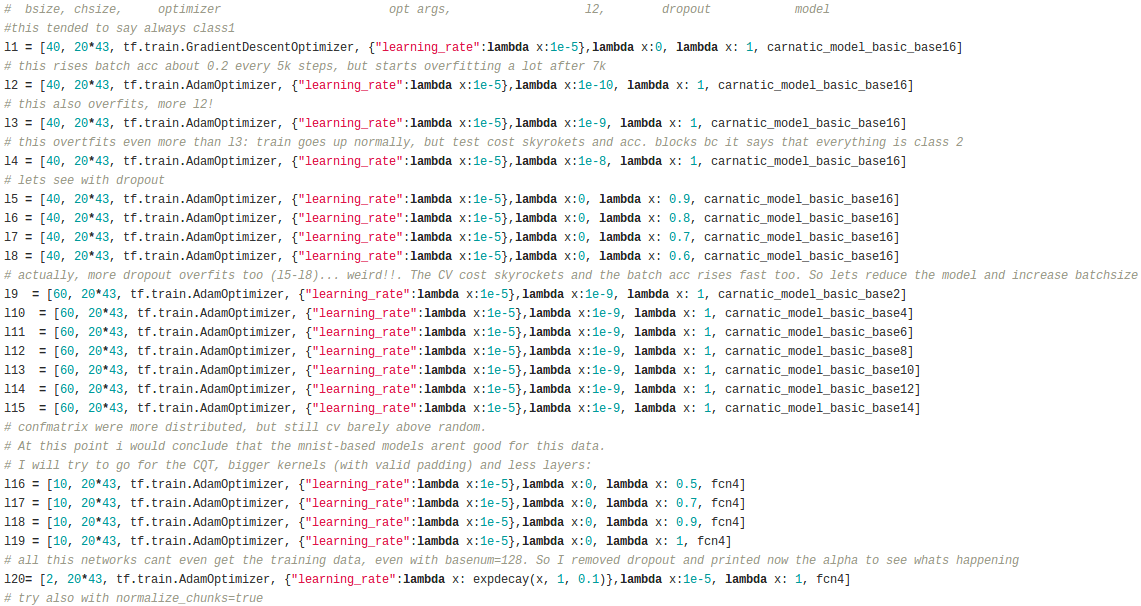
\includegraphics[scale=0.37]{finetuning_caption.png}
  \end{frame}



  \begin{frame}
    \frametitle{$RRD$ -- Confusion Matrix Example}
    \centering
    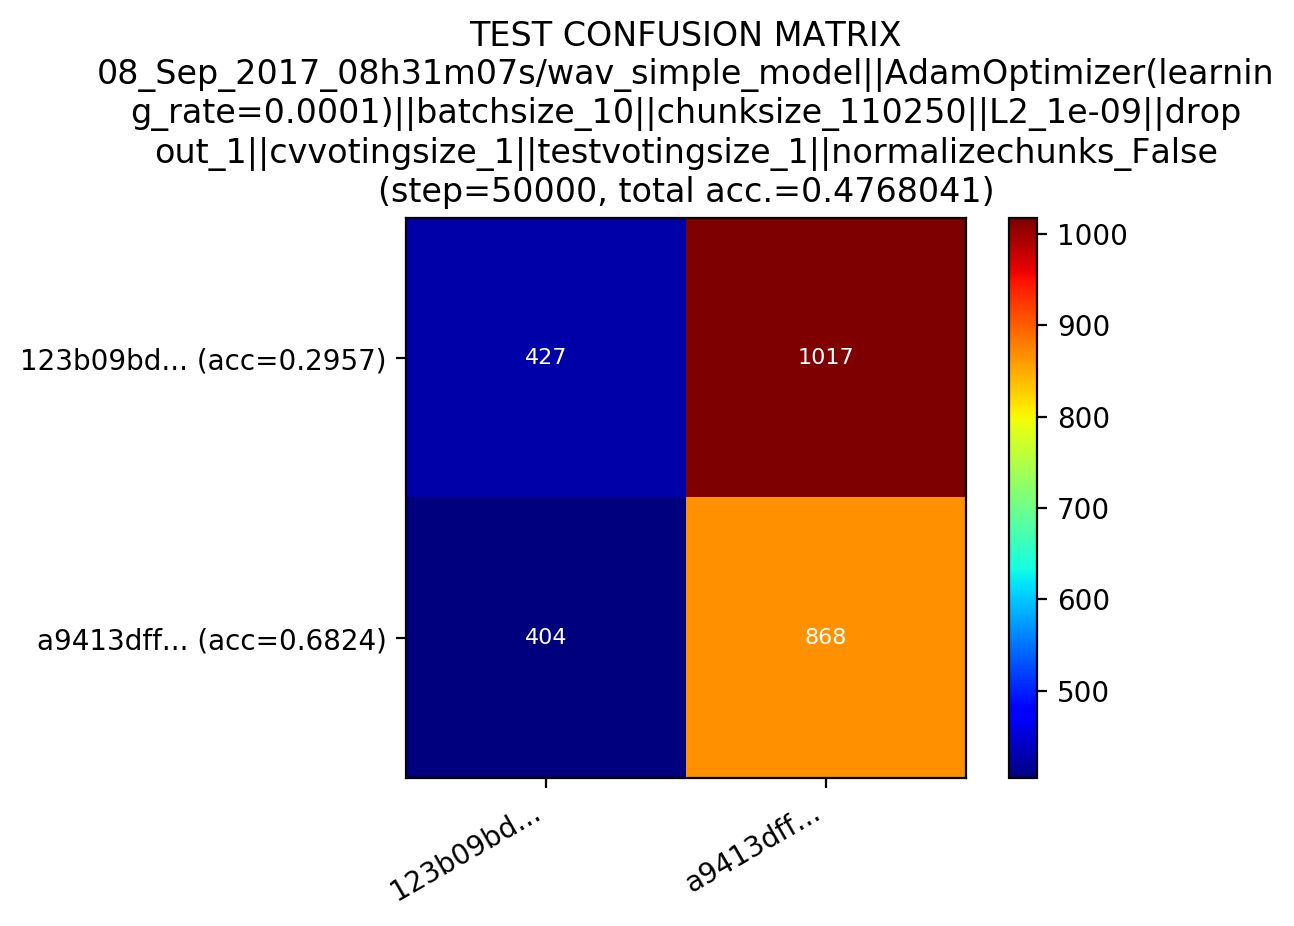
\includegraphics[scale=0.18]{confmat_class2.png}
    \begin{block}{}
      An examination of the confusion matrices shows that the model is learning orthogonally to the classification boundary, that is, features that don't play a role in r\=aga classification.
    \end{block}
  \end{frame}


     %%%%%%%%%%%%%%%%%%%%%%%%%%%%%%%%%%%%%%%%%%%%%%%%%%%%%%%%%%%%%%%%%%%%%%%%%%%%%%%%%%%%%%%%
     \section{Conclusions and Follow-Up}
     \frame{\sectionpage}
     %%%%%%%%%%%%%%%%%%%%%%%%%%%%%%%%%%%%%%%%%%%%%%%%%%%%%%%%%%%%%%%%%%%%%%%%%%%%%%%%%%%%%%%%

     \begin{frame}
       \frametitle{Conclusions and Follow-up}
       \begin{itemize}
       \item \Large Conclusions:
         \begin{enumerate}
         \item The chosen time/frequency representations are probably too sparse to allow any kind of regularization to be effective
         \item basic preprocessing like cutting off non-melodic segments would have been instrumental
         \item Histograms of the network weights would have helped the diagnose
         \end{enumerate}
         \vspace{5mm}
       \item \Large Follow-up:
         \begin{enumerate}
         \item Train similar networks on the TDMS to confirm data issue
         \item Incorporating the TDMS to other problem domains (f.e. western MGR)
         \item Implementing the auralization technique\cite{choi-explaining} (a sort of deconvolution for audio) as a diagnose tool to get a beter insight on the networks' problems
         \end{enumerate}
       \end{itemize}
     \end{frame}

     
     \begin{frame}
       \begin{center}
         \Large \textbf{THANK YOU}\\[20pt]
         
       Questions?
       \end{center}
     \end{frame}
       

     %%%%%%%%%%%%%%%%%%%%%%%%%%%%%%%%%%%%%%%%%%%%%%%%%%%%%%%%%%%%%%%%%%%%%%%%%%%%%%%%%%%%%%%%
     \appendix
     \section{Bibliography}
     % \frame{\sectionpage}
     %%%%%%%%%%%%%%%%%%%%%%%%%%%%%%%%%%%%%%%%%%%%%%%%%%%%%%%%%%%%%%%%%%%%%%%%%%%%%%%%%%%%%%%%

     \begin{frame}[c] % [plain, c]
       \begin{center}
         \LARGE Bibliography
       \end{center}
     \end{frame}

     
     \begin{frame}[allowframebreaks]
       \bibliographystyle{apalike}
       \tiny \printbibliography
     \end{frame}

\end{document}




%% \begin{frame}\frametitle{lists with single pauses}
%%   \begin{itemize}
%%   \item Introduction to  \LaTeX{}  \pause 
%%   \item Course 2 \pause 
%%   \item Termpapers and presentations with \LaTeX{}  \pause 
%%   \item Beamer class
%%   \end{itemize} 
%% \end{frame}

%% \begin{frame}\frametitle{lists with pause}
%%   \begin{itemize}[<+->]
%%   \item Introduction to  \LaTeX{}  
%%   \item Course 2
%%   \item Termpapers and presentations with \LaTeX{}  
%%   \item Beamer class
%%   \end{itemize} 
%% \end{frame}

%% \begin{frame}
%%   \frametitle{numbered lists with single pauses}
%%   \begin{enumerate}
%%   \item Introduction to  \LaTeX{}  \pause 
%%   \item Course 2 \pause 
%%   \item Termpapers and presentations with \LaTeX{}  \pause 
%%   \item Beamer class
%%   \end{enumerate}
%% \end{frame}

%% \begin{frame}
%%   \frametitle{numbered lists with pause}
%%   \begin{enumerate}[<+->]
%%   \item Introduction to  \LaTeX{}  
%%   \item Course 2
%%   \item Termpapers and presentations with \LaTeX{}  
%%   \item Beamer class
%%   \end{enumerate}
%% \end{frame}
